% 2005 年湖北卷理科第 10 题配图：三棱柱 ABC-A'B'C' 与点 E, F, H, K, G
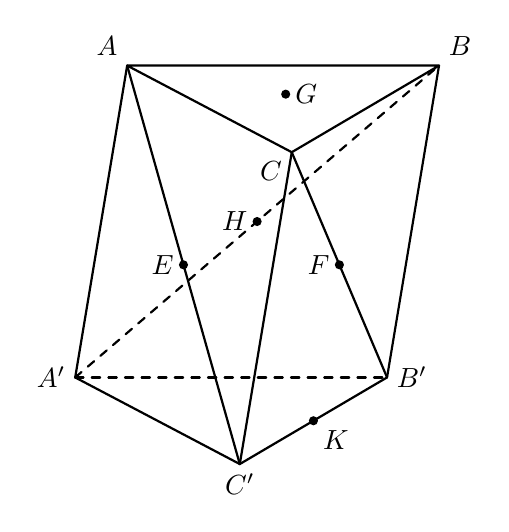
\begin{tikzpicture}[>=stealth,scale=1.1,line cap=round,line join=round]
  % 顶点坐标
  \coordinate (A) at (0,3.0);
  \coordinate (B) at (3.6,3.0);
  \coordinate (C) at (1.9,2.0);
  \coordinate (A1) at (-0.6,-0.6);
  \coordinate (B1) at (3.0,-0.6);
  \coordinate (C1) at (1.3,-1.6);

  % 中点与重心坐标
  \coordinate (G) at (1.83,2.67);
  \coordinate (E) at (0.65,0.7);
  \coordinate (F) at (2.45,0.7);
  \coordinate (H) at (1.5,1.2);
  \coordinate (K) at (2.15,-1.1);

  % 虚线不可见棱与对角线
  \draw[dashed,thick] (A1) -- (B1);
  \draw[dashed,thick] (A1) -- (B);

  % 实线可见棱
  \draw[thick] (A) -- (B) -- (C) -- cycle;
  \draw[thick] (A) -- (A1);
  \draw[thick] (B) -- (B1);
  \draw[thick] (C) -- (C1);
  \draw[thick] (A1) -- (C1) -- (B1);

  % 面对角线
  \draw[thick] (A) -- (C1);
  \draw[thick] (C) -- (B1);

  % 特殊点绘制
  \fill (G) circle (1.5pt) node[right] {$G$};
  \fill (E) circle (1.5pt) node[left] {$E$};
  \fill (F) circle (1.5pt) node[left] {$F$};
  \fill (H) circle (1.5pt) node[left] {$H$};
  \fill (K) circle (1.5pt) node[below right] {$K$};

  % 顶点标签
  \node[above left] at (A) {$A$};
  \node[above right] at (B) {$B$};
  \node[below left] at (C) {$C$};
  \node[left] at (A1) {$A'$};
  \node[right] at (B1) {$B'$};
  \node[below] at (C1) {$C'$};
\end{tikzpicture}
